\cotefile{156-8}
\scanpage{74}
\mspage{65}
% archive sheet number: 74

\unsure{Il} est temps de revenir aux supports \unsure{internes} dans un \unsure{magma}.

Utilisant la relation $\mid\circ\mid$ symétrique et antiréflexive, on trouve comme d'habitude, dans $\unsure{\mathcal{P}|P}(M)$, \deleted{\unsure{donc}} une opération
\[
\operatorname{cosupp}^{\circ}(A)=\{\deleted{\unsure{X|Y}}\unsure{Y|X}\in M\mid A\mid\circ\mid\deleted{\unsure{X|Y}}\unsure{Y|X}\deleted{\unsure{\}}}\quad\text{i.e.}\ \inserted{\forall X\in A,}\ X\mid\circ\mid Y\}
\]
où on pose, pour deux parties $A,B$ de $M$
\[
 A\mid\circ\mid B\ \overset{\mathrm{def}}{\Longleftrightarrow}\ \forall X\in A,\ Y\in B,\ \text{on a :}\ X\mid\circ\mid Y
\]
et
\[
 A\mid\circ\mid X\ \overset{\mathrm{def}}{\Longleftrightarrow}\ A\mid\circ\mid\{X\}.
\]
\deleted{\unsure{On po|On a}}
On \deleted{\unsure{peut écrire}} a
\deleted{\unsure{Ainsi} $\operatorname{cosupp}^{\circ}$}
\[
\left\{\begin{aligned}
\operatorname{cosupp}^{\circ}(\textstyle\bigcup A_i)&=\bigcap_i\operatorname{cosupp}^{\circ}(A_i)\\
\operatorname{cosupp}^{\circ}(\varnothing_M)&=\deleted{\operatorname{cosupp}^{\circ}(\unsure{\{\varnothing\}})}M\\
\operatorname{cosupp}^{\circ}(M)&=\varnothing
\end{aligned}\right.
\]
On pose
\[
\operatorname{supp}^{\circ}(\deleted{\unsure{X}}A)=\operatorname{cosupp}^{\circ}(\operatorname{cosupp}^{\circ}(\deleted{\unsure{X}}A))
\]
% margin note written slanted
\margin{On pose\\$\operatorname{supp}^{\circ}(X)=\operatorname{supp}^{\circ}(\{X\})$\\$\operatorname{cosupp}^{\circ}(X)=\operatorname{cosupp}^{\circ}(\{X\})$}
On dit qu'une partie \inserted{$S$} de $M$ est un $\mid\circ\mid$-support, si elle est de la forme $\operatorname{supp}^{\circ}(A)$, ou ce qui revient au $=$, si on a
\[
 A=\operatorname{supp}^{\circ}(A)
\]
Notons qu'une telle partie est fermée pour $\overset{\circ}{\ll}$ :
\[
 X\in A,\quad X'\overset{\circ}{\ll}X\quad\Rightarrow\quad X'\in A.
\]
Mais elle n'est pas \unsure{néc.} fermée pour $\leq$, et encore moins pour $\ll$. \deleted{\unsure{Ce}}

La relation avec la notion précédente de \uline{support} (pour $\mathrel{\|}$), \deleted{\unsure{d'une partie}} est
\scanpage{75}
\mspage{66}
% archive sheet number: 75

la suivante :
\[
\begin{aligned}
\operatorname{cosupp}X&=\inserted{\{Y\in M\mid\widetilde{Y}\subset}\operatorname{cosupp}^{\circ}(\widetilde{X})\inserted{\}}\\
\operatorname{cosupp}A&=\inserted{\{Y\in M\mid\widetilde{Y}\subset}\operatorname{cosupp}^{\circ}(\widetilde{A})\inserted{\}}
\end{aligned}
\]
(où $\widetilde{A}\overset{\mathrm{def}}{=}\bigcup_{X\in A}\widetilde{X}$ (\deleted{\unsure{saturée de}}\inserted{plus petite} partie fermée de $M,\leq$ contenant $A$)

\deleted{Donc $\operatorname{cosupp}A=\operatorname{cosupp}^{\circ}(A)$ si $A=\widetilde{A}$ i.e. $A$ fermé dans $M$ pour $\leq$.}
% margin note written slanted
\margin{\uline{idiot}}

% Two long oblique cancellation strokes cross the following block.
\deleted{\unsure{En.} Ainsi, les supports sont les supports \unsure{internes} des parties de $M$ \uline{fermées} pour $\leq$. En effet, pour une telle partie, prendre $\operatorname{cosupp}^{\circ}$ ou $\operatorname{cosupp}$ revient au $=$ et le résultat est $\leq$-fermé, et \unsure{le réappliquant}, on trouve l'assertion.}

\deleted{Le traitement précédent des supports était vicié par le fait, qu'il ne travaillait \inserted{seulement} \deleted{\unsure{au démarrage}} qu'avec les supports des parties fermées.} Les $\operatorname{supp}$ et $\operatorname{cosupp}.$ s'expriment, on l'a vu, en termes des $\operatorname{supp}^{\circ}$ et $\operatorname{cosupp}^{\circ}$, mais l'inverse n'est pas vrai.

\uline{Exemple instructif} : \unsure{magma} trivial\inserted{\unsure{ou n'importe,}}. La relation $\mid\circ\mid$ est la relation $X\ne Y$. Donc les supports sont les parties quelconques de $M$. Je peux visualiser une telle partie $A$, comme représentant la réunion des ``\uline{cellules ouvertes}'' $X^{\circ}$, pour $X\in A$. Si on
\scanpage{76}
\mspage{67}
% archive sheet number: 76

travaille avec la relation $X\mathrel{\|}Y\Longleftrightarrow\widetilde{X}\cap\widetilde{Y}=\varnothing$, les supports sont \uline{certaines} parties fermées de $M,\leq$ bien particulières. \unsure{Jamais par} elles on ne pourra exprimer des supports internes !

Je désigne par $\Sigma_M$ (notation \unsure{standard|standart}) \unsure{l'ens} des supports pour $M$. \deleted{L'application} Cet ensemble, \deleted{\unsure{est|et}} ordonné par $\subset$, a un plus petit élément $\varnothing$, et un plus grand élément $M$. Il a des $\operatorname{Inf}$ quelconques -- ce sont les $\bigcap_i$ simplement. Il y a une \deleted{fonction} application
\[
\Sigma_M\overset{\sim}{\longrightarrow}\Sigma_M\qquad S\longrightarrow\deleted{\unsure{C}}\unsure{\complement|C}S,
\]
qui est une antiinvolution de l'ens ordonné. Il \deleted{\unsure{tr}} transforme des $\operatorname{Inf}$ en $\operatorname{Sup}$ et inversement. Le $\operatorname{Sup}$ s'écrit aussi
\[
\operatorname{Sup}S_i=\operatorname{supp}^{\circ}(\textstyle\bigcup S_i)
\]
On prendra bien garde de ne pas \unsure{le|les} confondre avec $\bigcup S_i$.

On peut aussi construire un $\Sigma_L$, avec $\mid\circ\mid_L=\mathrel{\|}_L$ sur $L$. On \deleted{\unsure{trouvera}}\inserted{voudrait} une application canonique
\scanpage{77}
\mspage{68}
% archive sheet number: 77

\[
\Sigma_M\longrightarrow\Sigma_L\qquad S\longrightarrow S\cap L
\]
mais est-on sûr que si $S$ est un support\inserted{(interne)}, $S\cap L$ en soit un ? C'est OK si on suppose Mag L 2 \deleted{\unsure{qui} \illegible{2} \unsure{dans le cas quasi-accessible}} \inserted{(\unsure{magmas Art. dirigibles|magmas Art. divisibles})}, car alors,
\[
\operatorname{cosupp}^{\circ}_M X=\operatorname{cosupp}^{\circ}_M(\operatorname{omb}^{\circ}X)
\]
% margin note written slanted
\margin{NB. On en conclut\\$\operatorname{supp}^{\circ}X=\operatorname{supp}^{\circ}(\operatorname{omb}^{\circ}X)$}
et plus généralement, pour une partie quelc. $A$ de $M$
\[
\operatorname{cosupp}^{\circ}_M(A)=\operatorname{cosupp}^{\circ}_M(\operatorname{omb}^{\circ}(A))
\]
où on pose
\[
\operatorname{omb}^{\circ}(A)=\bigcup_{X\in A}\operatorname{omb}^{\circ}(X)\subset L
\]
on en conclut
\[
\operatorname{cosupp}^{\circ}_M(A)\cap L=\operatorname{cosupp}^{\circ}_L(\operatorname{omb}(A)),
\]
\deleted{\unsure{donc}} ce qui prouve que si $S$ est un support\inserted{(interne)} dans $M$ i.e. de la forme $\operatorname{cosupp}^{\circ}_M(A)$, alors $S\cap L$ est un support (interne) dans $L$.

On trouve une application en sens inverse
\[
\begin{aligned}
\Sigma_L&\longrightarrow\Sigma_M\\
 A&\longrightarrow\operatorname{supp}^{\circ}_M(A)\underset{\uparrow}{\overset{?}{=}}\{X\in M\mid\operatorname{omb}^{\circ}X\subset A\unsure{)|\}}
\end{aligned}
\]
A-t-on bien l'égalité annoncée ? Sûrement, si
\[
\inserted{X\in M}\ \deleted{\unsure{si}}\quad\operatorname{omb}^{\circ}(X)\subset A\quad\Rightarrow\quad
\underset{\inserted{\substack{\Vert\\\operatorname{supp}^{\circ}(\operatorname{omb}^{\circ}(X))}}}{\deleted{\unsure{\operatorname{supp}}}\operatorname{supp}^{\circ}(X)}
\unsure{\subset|\in}\operatorname{supp}^{\circ}_M(A)
\]
d'où $X\in\deleted{\unsure{\operatorname{cosupp}}}\operatorname{supp}^{\circ}_M(A)$. Mais inversement, supposons
\scanpage{78}
\mspage{69}
% archive sheet number: 78

$X\in\operatorname{supp}^{\circ}_M(A)$, on en conclut (puisque $\operatorname{supp}^{\circ}$ est fermé pour $\overset{\circ}{\ll}$) $\operatorname{omb}^{\circ}(X)\subset\operatorname{supp}^{\circ}_M(A)$, OK.

Ceci dit, les deux applications précédentes sont inverses l'une de l'autre, et établissent des iso. réciproques d'ens. ordonnés, munis de l'opération $\unsure{\complement|C}\ldots$

C'est formel en termes de
\diagram{\begin{tikzcd}[ampersand replacement=\&,row sep=2em,column sep=4em]
 L \arrow[d,hook] \arrow[dr,"x\mapsto\{x\}"] \arrow[dr,phantom,"\text{comm.}"{description,pos=.6,xshift=-15pt,yshift=-10pt}] \& \\
 M \arrow[r] \& \unsure{\mathcal{P}|P}(L)
\end{tikzcd}}
application (ici $X\mapsto\operatorname{omb}^{\circ}(X)$), $\mathrel{\|}_L$ relation sym. antiréfl. sur $L$ d'où relation $\mid\circ\mid_M$ sur $M$ par
\[
 X\mid\circ\mid Y\Longleftrightarrow o(X)\mathrel{\|}o(Y)
\]
i.e. $\forall x\in o(X),y\in o(Y),\ x\mathrel{\|}_L y$.
% margin note written slanted
\margin{On peut généraliser au cas d'une relation entre deux \uline{ens.} \uline{distincts} $M,M'$ versus $L,L'$, avec deux diagrammes au \deleted{\unsure{un}} lieu d'un, \unsure{fibré|figé}.}

% Several diagonal strokes cancel the following sentence and formula.
\deleted{À toute partie\inserted{$A$} \deleted{\unsure{de}} $\operatorname{supp}^{\circ}$ de $L$, on \unsure{associe} une partie\inserted{$\operatorname{supp}^{\circ}$} de $M$, par}
\[
\deleted{\unsure{\varphi|\phi}(A)=\{X\in M\mid o(X)\subset A\}}
\]
et on trouve \deleted{\unsure{ainsi}}\inserted{alors} deux iso \deleted{\unsure{tr}} réciproques.
\diagram{\begin{tikzcd}[ampersand replacement=\&]
\Sigma_L \arrow[r,shift left=.6ex] \& \Sigma_M \arrow[l,shift left=.6ex]
\end{tikzcd}}
\hfill $\ldots$

Il faudra bien que je me tape l'énoncé général, avec la vérification !

\uline{Cor} Si $\mathrel{\|}_L$ est la relation $x\ne y$ (cas \unsure{quasi-irréductible}) alors
\[
\Sigma_M\simeq\mathcal{P}(L)
\]
La notion de support\inserted{interne} est limpide : $\operatorname{supp}^{\circ}A$ s'identifie à $\operatorname{omb}^{\circ}(A)$.
\scanpage{79}
\mspage{70}
% archive sheet number: 79

Si je me fatigue à faire une théorie ``abstraite'', c'est bien sûr pour pouvoir parler des supports aussi en dehors du cas \unsure{quasi-accessible} (p. ex. pour les \unsure{cordes|cadres} \unsure{etc.}\unsure{\ldots})

Supposons qu'on ait une fonction support externe \uline{fidèle}
\[
 M\longrightarrow\unsure{\mathcal{P}|P}(P)\qquad X\longmapsto|X|
\]
% margin note written slanted; short pointers link it to the support application
\margin{mais \unsure{cette fois} on n'a pas d'appl $P\longrightarrow M$ !, cas général !}
(p. 62), j'ai envie \unsure{alors} de définir un \deleted{application injective, \unsure{comp}}\inserted{plongement}
\[
 \Sigma_M\subset\mathcal{P}(P)
\]
de telle façon que la relation d'ordre de $\Sigma_M$ soit induite par celle de $\mathcal{P}(P)$, que $\Sigma_M$ soit stable par $\operatorname{Sup}$ et $\operatorname{Inf}$ quelconques, et commute à $\unsure{\complement|C}$. Si on suppose $|M|=P$. Est-ce trop espérer ?

% Four long diagonal cancellation strokes cross the following unfinished block.
\deleted{Si $A\subset M$, définissons}
\[
\deleted{|A|^{\circ}=\bigcup_{X\in A}|X|^{\circ}}
\]
\deleted{Donc si $A,B\subset M$, on a}
\[
\deleted{A\unsure{\}|\{}}
\]
\scanpage{80}
\mspage{71}
% archive sheet number: 80

Je regarde l'application
\[
 \unsure{\varphi|\phi}:X\longmapsto|X|^{\circ}\qquad M\longrightarrow\unsure{\mathcal{P}|P}(P),
\]
plus ``fine'' que $X\longmapsto|X|$. Par hypothèse la relation $\mid\circ\mid$ sur $M$ se déduit de la \deleted{\unsure{appl}} relation $x\ne y$ sur $P$, via l'application précédente. Je pose donc pour toute partie $A$ de $M$
\[
 |A|^{\circ}\ \text{ou}\ \varphi(A)\overset{\mathrm{def}}{=}\bigcup_{X\in A}\varphi\underbrace{(X)}_{|X|^{\circ}}
\]
et on trouve par hyp.
\[
 A\mathrel{\|}B\quad\Longleftrightarrow\quad\underbrace{\varphi(A)}_{S}\cap\varphi(B)=\varnothing
\]
Ceci vu, on aura donc
\[
 \operatorname{cosupp}^{\circ}(A)=\{\deleted{\unsure{B|X}}X\in M\mid\deleted{\unsure{\varphi(A)\mathrel{\|}X}}X\subset P\setminus\varphi(A)\}
\]
Par suite, on a
\[
 \varphi(\underbrace{\operatorname{cosupp}^{\circ}(A)}_{S})\subset P\setminus\varphi(A)
\]
et \inserted{la partie \deleted{\unsure{fermée}} support} $\underbrace{\operatorname{cosupp}^{\circ}(A)}_{S}$ est connue quand on connaît \deleted{$\unsure{\varphi(S)\subset}$} la partie $\varphi(S)=\deleted{\unsure{P}}$ de $P$ (et $\unsure{=|\subset|\ne}$ \unsure{à|de} $P\setminus\varphi(A)$), car
\[
 X\in S\Longleftrightarrow\varphi(X)\subset\varphi(S)
\]
\deleted{Donc l'application}

[En effet, $\Rightarrow$ tautologique, et $\Leftarrow$ car $\varphi(X)\subset\varphi(S)$ implique $\varphi(X)\subset P\setminus\varphi(A)$ i.e. $\varphi(X)\cap\varphi(A)=\varnothing$ i.e. $X\mid\circ\mid A$ donc $X\in\operatorname{cosupp}^{\circ}A$).

Ainsi l'application
\scanpage{81}
\mspage{72}
% archive sheet number: 81

\[
\begin{aligned}
 \Sigma_M&\longrightarrow\unsure{\mathcal{P}|P}(P)\\
 S&\longmapsto\unsure{\varphi|\phi}(S)\ (=|S|^{\circ})
\end{aligned}
\]
est injective, on trouve \unsure{un|une} inverse à gauche en associant, à toute partie $Q\deleted{\unsure{\subset}}$ de $P$, l'ens
\[
 \deleted{\unsure{S_Q=}}\quad\{X\in M\mid\varphi(X)\subset Q\}
\]
ou plutôt (comme celui-ci n'est peut-être pas lui-même un $\operatorname{supp}^{\circ}$)
\[
 S_Q=\operatorname{supp}^{\circ}(\{X\in M\mid\varphi(X)\subset Q\}).
\]

Est-on déraisonnable, d'espérer que le plongement précédent commute $\unsure{\rightleftarrows|\complement}$, i.e. qu'on puisse y comprendre quelque chose aux supports\inserted{intrinsèques} des figures (élémentaires en l'occurrence) qui ne soit \deleted{pas} ni compatible, ni ne le devienne après subdivisions.
% margin note written slanted
\margin{Il ne commute pas aux $A\cap B$ déjà dans le cas de la \unsure{réalis.} tautologique \unsure{d'un|d'une} \unsure{cadre|corde} topologique pour les supports associés à deux ``cellules'', cf \unsure{figure}.}
% Drawing in the left margin, below the slanted note.
\figure{
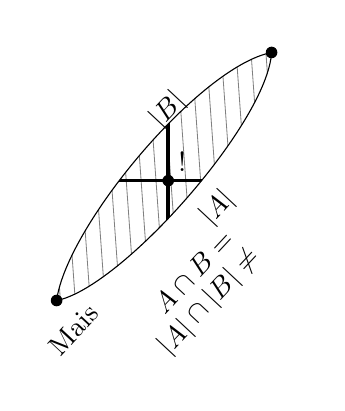
\begin{tikzpicture}[scale=1.05]
\path[use as bounding box] (-.35,-1.0) rectangle (3.15,3.3);
\begin{scope}
\clip (0,0) .. controls (.12,.9) and (1.73,2.83) .. (2.6,3.0) .. controls (2.55,2.15) and (.78,.15) .. (0,0);
\foreach \x in {-0.3,-0.12,0.06,0.24,0.42,0.60,0.78,0.96,1.14,1.32,1.50,1.68,1.86,2.04,2.22,2.40,2.58,2.76}{\draw[gray,line width=.3pt] (\x,-.2)--(\x-.25,3.3);}
\draw[line width=1.3pt] (.7,1.45)--(1.95,1.45);
\draw[line width=1.3pt] (1.35,.75)--(1.35,2.2);
\end{scope}
\draw (0,0) .. controls (.12,.9) and (1.73,2.83) .. (2.6,3.0) .. controls (2.55,2.15) and (.78,.15) .. (0,0);
\fill (0,0) circle (2pt) (2.6,3.0) circle (2pt) (1.35,1.45) circle (2pt);
\node at (1.52,1.68) {!};
\node[rotate=47] at (1.35,2.3) {$|B|$};
\node[rotate=47] at (1.95,1.12) {$|A|$};
\node[rotate=47] at (.2,-.35) {\deleted{\unsure{Mais}}};
\node[rotate=47] at (1.65,.35) {$A\cap B=\varnothing$};
\node[rotate=47] at (1.85,-.02) {$|A|\cap|B|\ne\varnothing$};
\end{tikzpicture}}

Aussi faudrait-il à présent que je me limite à des supports de nature très particulière, \unsure{attachés} à une figure (supports ``constructibles'')
